%!TEX root = Thesis_David_Burns.tex
\chapter{Analysis and Discussion}
\label{ch:analdisc}

%-----------------------------------------------------------------------------------------------------------------
%------------------------------------------------------------------------------------------------------------------
\section{HYSPLIT Modelling}
\label{sec:hysplitwork}

	%------------------------------------------------------------------------------------------------------------------
	\subsection{Assessing Locations and Months}
	\label{subsec:asslocs}

	The interpolated histograms in \cref{sec:hysplitresults} show a general trend of air packets coming from the Pacific Ocean and towards the coast. The direction of wind vectors in \cref{fig:windmap}, modelled in \gls{ccam} agrees, with a majority pointing in the westerly direction. This indicates that almost year round, at locations along the Queensland coast, the majority of the air packets that arrive there have passed over the \gls{gbr}. There are identifiable differences between locations and months that determine suitability for coastal experimental locations and ship routes.

	Looking at \cref{fig:gbrboundary}, the reef runs right down the Queensland coast, but the coast begins to jut out to the east at around \ang{20} S. This creates a section of the reef running more to the east-southeast, matching the wind direction. The reef also widens into the Swain Reefs creating a larger body. Selecting locations and months where the interpolated histograms show a large proportion of air packets coming over that stretch of reef provides the highest chance of detecting the reefs output of \gls{dms}. It is also important that as little as possible originates from the land, as anthropogenic sources would mask the reef sources. In \cref{fig:comphisto} there are examples of this analysis for selecting suitable and unsuitable locations and months.

	\begin{figure}[!hbt]
    \centering
    \begin{subfigure}[b]{0.45\textwidth}
	    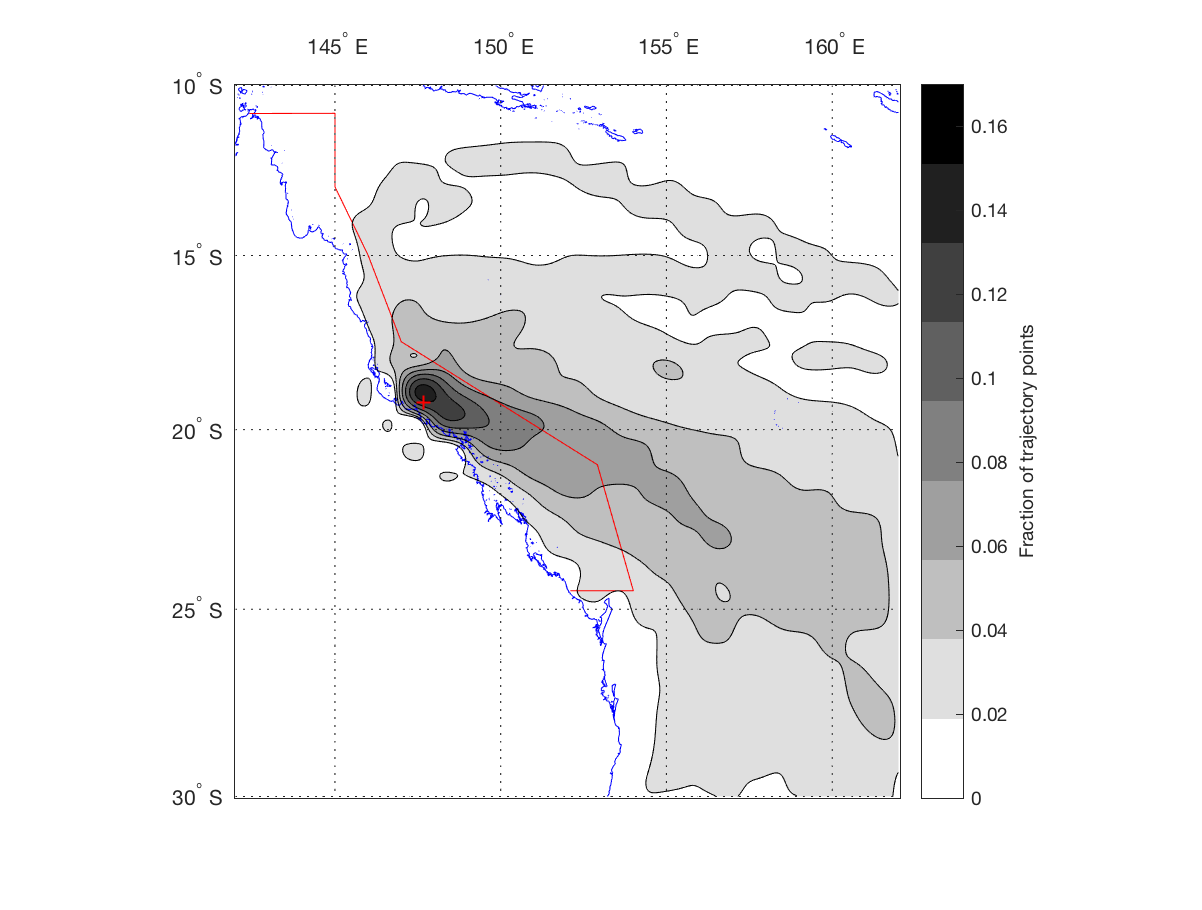
\includegraphics[width=\textwidth]{Fig/Research/BT_Ship/Map_103.eps}
	    \caption{October, Townsville -19.24, 147.67}
	    \label{subfig:octtown}
    \end{subfigure}
    ~
    \begin{subfigure}[b]{0.45\textwidth}
    	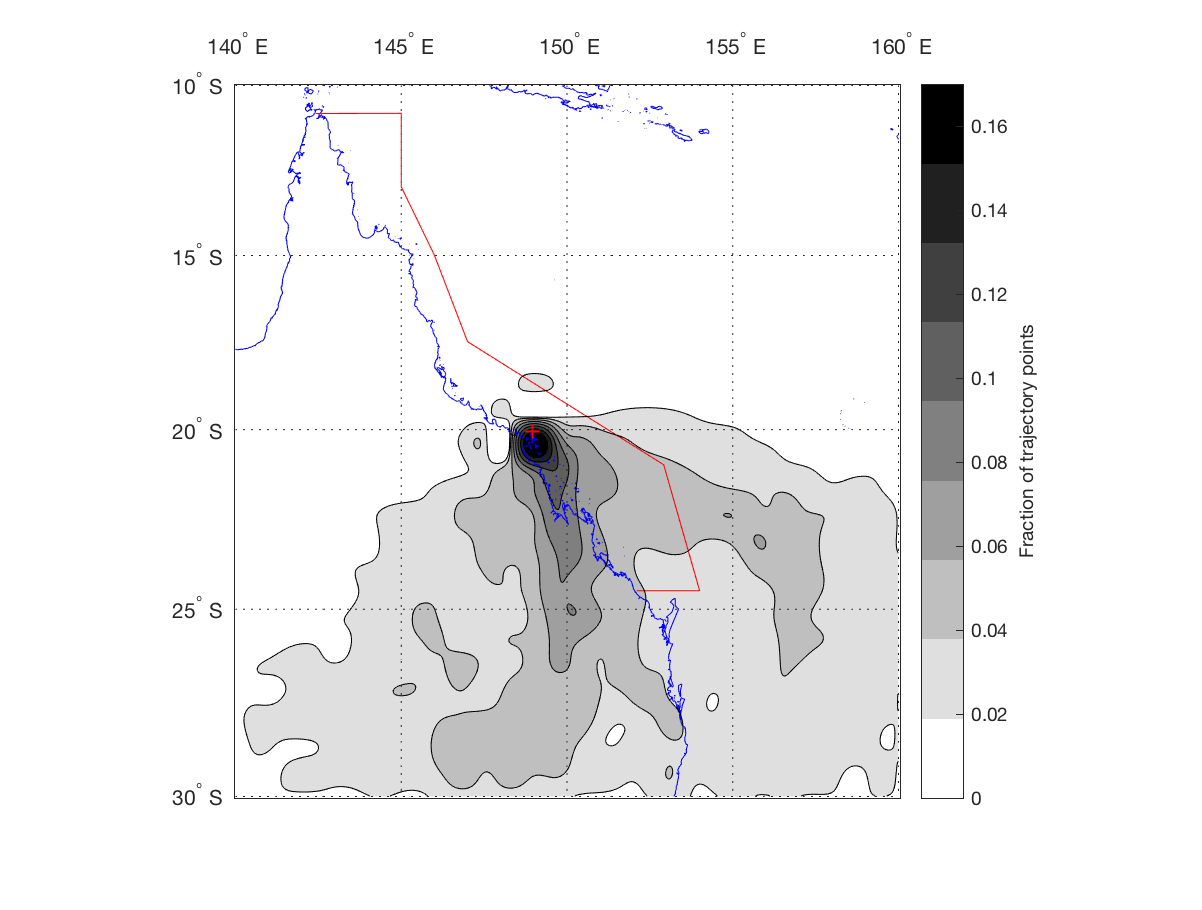
\includegraphics[width=\textwidth]{Fig/Research/BT_Coast/Map_062.eps}
	    \caption{June, Whitsundays -20.06, 148.95}
	    \label{subfig:junewhit}
    \end{subfigure}
    \caption{ A comparison of interpolated histograms of back trajectory points modelled six times daily, over the years 2011 to 2014. The locations and months are listed. An example of a suitable location and month, with the majority of the air travelling over a large section of the \gls{gbr} can be seen in \cref{subfig:octtown}. \Cref{subfig:junewhit} is an example of an unsuitable location, with the bulk source coming off the land. }
    \label{fig:comphisto}
	\end{figure}
	
	%------------------------------------------------------------------------------------------------------------------
	\subsection{Advising the Experimental Campaign}
	\label{subsec:expcamp}

	The best months appeared to occur in the later part of the year, September, October, and November. This was fairly consistent across all locations. October was the month selected for the experimental campaign, based on ship availability and this analysis. One of the coastal locations chosen was Mission Beach (-17.87 146.11). The location modelled in \cref{fig:chosenbtloc} is very close to this and shows a decent proportion of air packets coming off the reef, with little influence from the land.

	\begin{figure}[!htb]
    	\centering
    	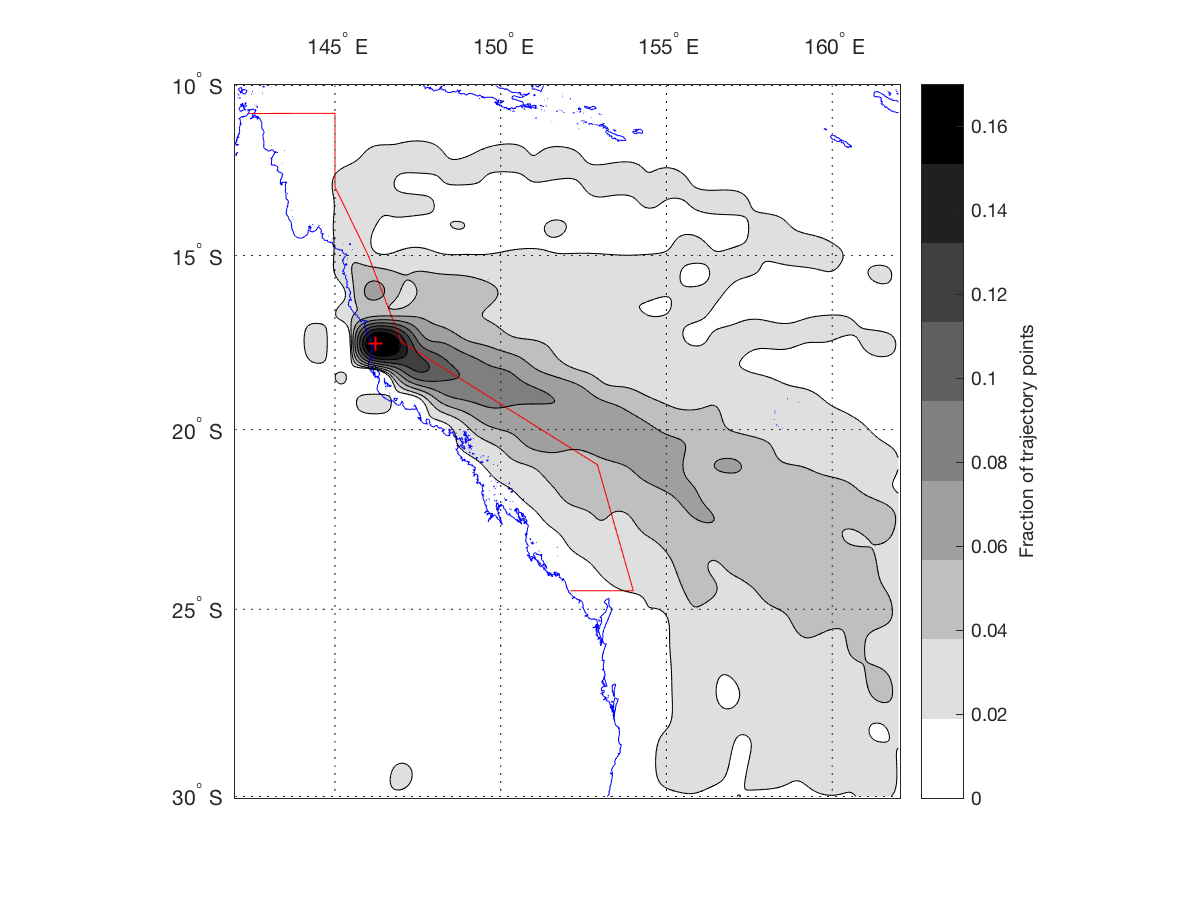
\includegraphics[width=0.8\textwidth]{Fig/Research/BT_Ship/Map_105.eps}
    	\caption{ Interpolated histograms of back trajectory points modelled six times daily, during October, over the years 2011 to 2014 at Innisfail (-17.533, 146.230). This is an example of a suitable location that was used in the campaign. }
    \label{fig:chosenbtloc}
	\end{figure}

	% Get a plot of the decided ship route in here.
\clearpage

%------------------------------------------------------------------------------------------------------------------
%------------------------------------------------------------------------------------------------------------------
\section{CCAM Modelling}
\label{sec:ccamwork}

	%------------------------------------------------------------------------------------------------------------------
	\subsection{Modelling of Meteorology Processes}
	\label{subsec:metproc}

	While \gls{ccam} doesn't model aerosols, and thus \gls{ccn}, it still produces cloud and rain data by assuming their presence. Humidity, pressure and temperature are used for generating cloud fractions. In \cref{fig:cldmap} and \cref{fig:rainmap} there are high levels of both total cloud fraction and rain along the Queensland coastline. Looking at the map of the surface height \cref{fig:zsmap} the same areas are low, almost sea level height regions, abutted by mountains. Moist warm air from the ocean moves inland and is pushed upwards by the increasing surface height. This cools the air without changing its water content causing condensation to occur (see \cref{subsec:relhum}). 

	The \gls{hysplit} work showed that most of the air coming from the Pacific Ocean to the coast. In \cref{fig:multiwind} the bottom pressure levels (highest values) show the east-west wind speed for most of the month as a negative value indicating an easterly wind (travelling towards the west). These easterly winds are the trade winds caused by a combination of the Hadley cell circulation and the Coriolis force \citep[Chapter 1]{seinfeld2012atmospheric}. The high, positive east-west wind speeds at the top pressure level is likely the top of the Hadley cell.

	% the multiple wind levels plot
	\begin{figure}[!htb]
	    \centering
	    \includegraphics[width=0.7\textwidth]{Fig/Research/CCAM/GBRAveragedPlot_multilevelwind.eps}
	    \caption{ The east-west Wind Speed, averaged from the points inside the \gls{gbr} region of the final \gls{ccam} domain. The 	highest, middle, and lowest pressure levels are shown. }
	    \label{fig:multiwind}
	\end{figure}

	An interesting meteorological event occurs over the \gls{gbr} towards the end of the month beginning on the 19th. This can be seen in \cref{fig:magwind} where the magnitude of the wind decreases from an average of \SI[per-mode=symbol]{8.77}{\meter\per\second} to an average of \SI[per-mode=symbol]{5.55}{\meter\per\second}. The opposite occurs to the temperature at the bottom pressure level (see \cref{fig:tbottime}), with an average of \SI{23.72}{\celsius} before the 19th rising to an average \SI{25.10}{\celsius} after the 19th. The cause of this shift is likely due to a pressure front moving through the \gls{gbr}. In \cref{fig:psltime} the mean sea level pressure can be seen dropping down to \SI{1014}{hPa} from \SI{1019}{hPa}. Winds move towards low pressure regions \citep{seinfeld2012atmospheric}. The low moves from west to east across the \gls{gbr} over the last part of the month countering the trade winds, decreasing the wind speed. This in turn increases the temperature over the \gls{gbr} as the winds transfer less of the solar heating of the reef away.

	%mean sea level
	\begin{figure}[!htb]
	    \centering
	    \includegraphics[width=0.7\textwidth]{Fig/Research/CCAM/GBRAveragedPlot_psl.eps}
	    \caption{ The Mean Sea Level Pressure, averaged from the points inside the \gls{gbr} region of the final \gls{ccam} domain. }
	    \label{fig:psltime}
	\end{figure}

	\clearpage

	%------------------------------------------------------------------------------------------------------------------
	\subsection{Influences on DMS Production}
	\label{subsec:dmsinfl}

	Both ocean temperatures and solar radiation levels effect the production of \gls{dmsp} by corals \citep{raina:2013fj}, \citep{fischer2012atmospheric}. In \cref{fig:tsutime} the surface temperature of the \gls{gbr} is plotted over time with an increase of \SI{1}{\celsius} towards the end of the month. The plots in \cref{fig:cldtime} and \cref{fig:rnettime} show a link between the amount of total surface radiation to total cloud fraction. This highlights the importance of local meteorology on surface temperature, and total surface radiation, the main influences on \gls{dms} production. 

	% The surface temp over gbr plot
	\begin{figure}[!htb]
	    \centering
	    \includegraphics[width=0.7\textwidth]{Fig/Research/CCAM/GBRAveragedPlot_tsu_ave.eps}
	    \caption{ The Surface Temperature, averaged from the points inside the \gls{gbr} region of the final \gls{ccam} domain. }
	    \label{fig:tsutime}
	\end{figure}

	In \cref{fig:magwind} the wind speed across the modelled region of the \gls{gbr} can be seen varying between \SIlist[per-mode=symbol]{3.5; 12}{\meter\per\second}. The wind speed varies quite drastically over the month with the last third of the month experiencing a prolonged decrease. The transfer of \gls{dms} from the ocean into the air depends heavily on the wind sheer at the surface (see \cref{sec:dmssurf}) \citep{Kettle:2000jy}. This indicates that the bulk of \gls{dms} moving into the atmosphere would also experience these fluctuations making it advisable to use a \gls{dms} surface flux model based on \gls{ccam}'s wind speed rather than directly feeding in \gls{dms} atmospheric concentrations.

	\clearpage

	%------------------------------------------------------------------------------------------------------------------
	\subsection{Limitations and Reliability of CCAM Data}
	\label{subsec:limitccam}

	The percentage difference was calculated between the \gls{ccam} and \gls{bom} values for the available variables and station locations. Taking the mean of these percentage differences over time (see \cref{eq:meanpd}) for each location provides an indicator for how well \gls{ccam} is simulating the interactions surrounding these atmospheric properties. These values measure the normalised distance allowing comparison with each other.
	
\begin{figure}[!hbt]
    \centering
    \begin{subfigure}[b]{0.45\textwidth}
    	\includegraphics[width=\textwidth]{Fig/Research/BomComparison/MaxTemp_PercentageDiffMean.eps}
	    \caption{}
	    \label{subfig:maxtlucpoint}
    \end{subfigure}
    ~~~
    \begin{subfigure}[b]{0.45\textwidth}
    	\includegraphics[width=\textwidth]{Fig/Research/BomComparison/MinTemp_PercentageDiffMean.eps}
	    \caption{}
	    \label{subfig:maxtladyelliot}
    \end{subfigure}
    \\
    \vspace{0.5cm}
    \begin{subfigure}[b]{0.45\textwidth}
        \includegraphics[width=\textwidth]{Fig/Research/BomComparison/MaxWind_PercentageDiffMean.eps}
	    \caption{}
	    \label{subfig:maxtlihoureef}
    \end{subfigure}
    \caption{The mean percentage differences and their standard deviations calculated by comparing the labelled measurement variables at a number of \gls{bom} station locations with the output of \gls{ccam}.}
    \label{fig:bomcompdata}
\end{figure}

	Looking at the values in \cref{tab:bommeanres}, the modelled temperature appears to be underestimating the maximum temperature and overestimating the minimum temperature. This may be a lack of variation in the model, however in \cref{fig:bomcompdata} the trend is fairly constant across the month. A similar problem effects wind speeds with \gls{ccam} under estimating the maximum wind speed. The mean percentage difference for maximum wind speed is quite high, around \SI{20}{\percent}. While the mean percentage difference for both temperatures is lower, this must be factored into any further modelling done using the \gls{ccam} data.









